\documentclass[10pt, conference, compsocconf]{IEEEtran}

% packages
\usepackage{algorithm}
\usepackage{algorithmic}
\usepackage{amsfonts} % for R symbol (the set of real numbers)
\usepackage{color}
\usepackage[pdftex]{graphicx}
\usepackage{graphicx}
\usepackage[bookmarks=false]{hyperref}
\hypersetup{colorlinks=true,linkcolor=black,citecolor=black,filecolor=black,urlcolor=blue}
\usepackage{mathtools}
\usepackage{multirow}
\usepackage{stmaryrd} % for llbracket and rrbracket
\usepackage{subcaption}
\usepackage{nicefrac}
\usepackage{amsmath}
\DeclarePairedDelimiter{\ceil}{\lceil}{\rceil}
\DeclarePairedDelimiter{\floor}{\lfloor}{\rfloor}

% new commands
\newcommand{\todo}[1]{\marginpar{\parbox{18mm}{\flushleft\tiny\color{red}\textbf{TODO}:
      #1}}}
\newcommand{\comment}[1]{\marginpar{\parbox{18mm}{\flushleft\tiny\color{blue}\textbf{Comment}:
      #1}}}

\newcommand{\note}[1]{
  \color{blue}\emph{[Note: #1]}
  \color{black}
}

\begin{document}

\title{Predicting computational reproducibility of scientific pipelines using collaborative filtering}

\author{Soudabeh Barghi, Lalet Scaria, Tristan Glatard\\
  Department of Computer Science and Software Engineering\\ Concordia University, Montreal, Quebec, Canada\\
  {first.last}@concordia.ca}

\maketitle

\begin{abstract}
\end{abstract}


\section{Introduction}

We consider the problem of predicting the values of a variable 
controlled by a hidden, parameterized, time dependent, deterministic 
process. We assume that the variable values are observed only for 
a limited number of time points, and we aim at predicting the values in the remaining time points.

We approach the problem from the point of view of collaborative 
filtering. The process is represented by a matrix where columns 
represent different parametrizations (we do not assume an order on the 
parametrizations) and rows represent the time points. The main difference with the traditional 
collaborative filtering problem 

% This is just a working example

Computational reproducibility, the property through which
computational results can be recomputed over time and
space~\cite{stodden}, has become a critical component of scientific
methodology with the rise of the reproducibility crisis in several
domains~\cite{xxx}. Among the factors hampering computational
reproducibility, infrastructural characteristics such as the operating
system play an important role. In neurosciences, our primary field of
interest, several studies have shown the effect of the operating
system on computational results. However, conducting such
reproducibility studies at scale is cumbersome due to the execution
time of data analysis pipelines, which easily exceeds a few hours.




In this paper we investigate approximate methods to predict the
reproducibility of a computational analysis from the first files that
it produces. Our main intuition is that reproducibility errors are
caused by a reduced number of factors that originate in the analysis
pipeline and input data. 

% Other possible examples

Seasonality of MS lesions.
Thresholded stock values. 

% Computational reproducibility is an issue, for instance among
% different operating systems (refer to Glatard FINF 2015,
% Gronenschild 2012).

% Scientific data analysis pipeline executions are long (give examples
% from neuroimaging).

% Refer to Germain et al 2008.

% Define subjects, pipelines.

% Problem: predict the reproducibility of pipeline files from other
% subjects and the first files produced by a pipeline. Restrict the
% study to binary classification.


\todo{Explain that columns represent subjects and rows represent files, and that these terms are used
indifferently}

\todo{Mention why this is Big Data}

\todo{Cite Cecile's paper}

\todo{Define reproducibility \emph{errors}}

\section{Method}

To evaluate the reproducibility of a pipeline, a retrieved matrix from 
the subjects and file-ids is built. Subjects and file-ids are equivalent 
to users and items, respectively, as they are known in Collaborative Filtering (CF) technique.
Filling in the missing entries of this matrix encompasses some issues 
which take some barriers for use of Collaborative filtering technique as it 
has being used in e-commerce applications.
For instance, files-ids (items) are produced in a specific order in the 
pipeline however items are sequentially independent in general use of CF in e-commerce.
This issue adds constraints on the selection of CF training set. Despite of random 
selection strategy which does not taking care of item order, we had to come up with those 
selection strategies that respect the pipeline fundamental fact about file order generation.  
The aforementioned matrix (utility matrix), con be fully completed by processing all subjects 
in pipeline however the whole processing can takes loads of time. This possibility of 
having a potential complete populated matrix means despite of potential sparse matrices 
in e-commerce case studies here the utility matrix is not sparse and 
we can decide precisely which samples we need to select as our training set selection. 
In this regard, to avoid the cold start issue we can take the first file-id of all 
subjects in order to get sure that for all subjects there is at least one 
selected element in training ratio and in the same way, all generated files 
from the process of a random subject which can guarantee that all files 
are presented in the selection set at least for once. 
 

 
what is specific to our problem compared to regular collaborative filtering:
%+ subjects are equivalent to users. Not all subjects have the same input data. Anatomical variability, acquisition variability (e.g., 1 subject may have multiple T1s).
%+ files are produced in a specific order (movies aren't),
% which add constraints on the training set (cannot sample late files and not early ones).
%+ utility matrix is not sparse: we can potentially populate it completely. Which means that we can decide precisely which samples we need (active sampling). Therefore we can take the first row and first column to avoid cold start issues.

\subsection{Collaborative filtering}

Collaborative filtering is a technique to predict unknown values of a 
matrix called ``utility matrix" from the known ones. Traditionally, the 
matrix represents the ratings of items, represented in columns, by 
users, represented in rows. Ratings might be explicit, when users 
provide ratings through a dedicated system, or implicit, when users' 
behaviors are tracked and analyzed to estimate their preferences. An 
overview of collaborative filtering is provided 
in~\cite{leskovec2014mining}.

Several methods have been proposed to implement collaborative 
filtering. Item-item collaborative filtering~\cite{breese1998empirical, linden2003amazon} predicts 
the rating of item $i$ by user $u$ from the ratings of items similar to 
$i$ by user $u$. Likewise, user-user collaborative 
filtering~\cite{breese1998empirical} predicts the rating of item $i$ by user $u$ 
from the ratings of item $i$ by users similar to $u$. Both methods
have been used extensively for e-commerce applications.

A third class of methods, which is the one we will apply to our 
problem, is based on the factorization of the utility matrix to 
estimate latent factors along which users and items are represented. 
This method is described 
in~\cite{koren2009matrix} and became famous as it contributed to winning the 
Netflix prize in 2009. To summarize, the method aims at finding $q_i$ 
and $p_u$ vectors of $\mathbb{R}^f$, where $f$ is the number of latent factors, such that:
\begin{equation*}
r_{ui} = q_i^Tp_u,
\end{equation*}
where $r_{ui}$ is the rating of item $i$ by user $u$. In practice, the optimization
involves a regularization term to avoid overfiting particular users or items. The method
finds $q_i$ and $p_u$ that minimize the following objective:
\begin{equation*}
\sum_{(i,u) \in \mathbb{T}}\left( r_{ui} - q_i^Tp_u\right)^2+\lambda \left( \|{q_i}\|^2 + \|{p_u}\|^2\right)
,
\end{equation*}
where $\lambda$ is the regularization parameter and $\mathbb{T}$ is the training set.

It is also common to include user biases $b_u$ and item biases $b_i$ in 
the optimization, defined as the average deviation of user $u$ and item 
$i$ to the global average $\mu$. The goal then becomes to find $q_i$ and $p_u$ that minimize the 
following objective:
\begin{equation*}
\sum_{(i,u) \in \mathbb{T}}\left( r_{ui} - \mu - b_u - b_i - q_i^Tp_u\right)^2+\lambda \left( \|{q_i}\|^2 + \|{p_u}\|^2 + b_u^2 + b_i^2\right)
\end{equation*}

Two good techniques to perform the optimization are stochastic gradient descent and alternating least squares (ALS). 
In the remainder of this paper, we use matrix factorization as implemented in 
Apache Spark's MLLib version 2.~\todo{xxx.}, which uses ALS.

% Explain our particular context.
% What our matrix represents
% Explain that you have binary classes (rounding)
% Explain the sampling issue.

\subsection{Sampling the training set}

As explained before, the training set in our problem cannot be 
constructed by unconstrained random sampling of the matrix.
To address this issue, we investigated the following sampling techniques. 

% 2. columns
\paragraph{Complete Columns (Figure~\ref{fig:Columns-Sample-Training-set})}
The training set is sampled by randomly selecting complete columns in
the matrix, that is, complete subject executions. The last selected
column might be incomplete to meet the exact training ratio. This 
method is realistic: it corresponds to a situation where the 
collaborative filtering method will predict the reproducibility in the 
remaining subjects from the subjects in the training set. 

% 3. rows
\paragraph{Complete Rows (Figure~\ref{fig:Rows-Sample-Training-set})} The training set is sampled by selecting complete 
rows in the matrix, that is, the first files produced by
every execution. The last selected row might be incomplete to meet the
exact training ratio. This method is realistic: it corresponds to a 
situation where the processing of all the subjects is launched and 
interrupted before the execution is complete. The collaborative 
filtering method will then predict the reproducibility of the remaining 
files.

\begin{figure}[h!]
        \centering
        \begin{subfigure}[b]{0.4\linewidth}
                  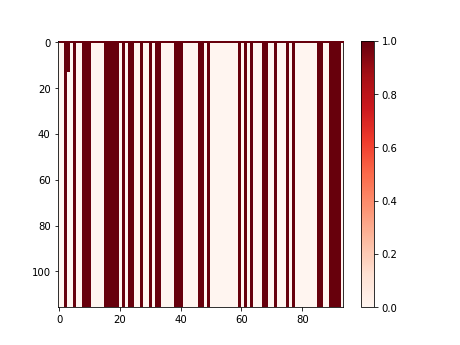
\includegraphics[width=\columnwidth]{figures/5vs7_columns_04_training}
                  \caption{Complete Columns}
                  \label{fig:Columns-Sample-Training-set}
        \end{subfigure}
        \begin{subfigure}[b]{0.4\linewidth}
                  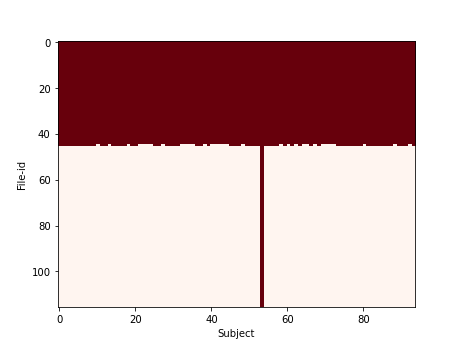
\includegraphics[width=\columnwidth]{figures/5vs7_rows_04_training}
                  \caption{Complete Rows}
                  \label{fig:Rows-Sample-Training-set}
        \end{subfigure}
        \begin{subfigure}[b]{0.4\linewidth}
                 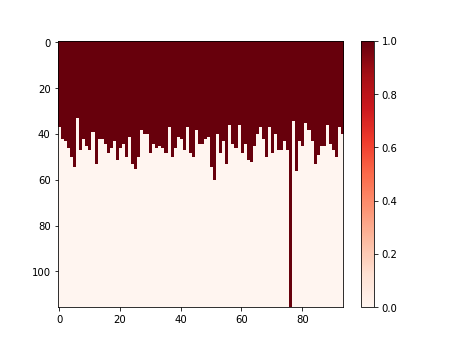
\includegraphics[width=\columnwidth]{figures/5vs7_random-real_04_training}
                \caption{Random Subjects (RS)}
                  \label{fig:Uniform-S-Sample-Training-set}
        \end{subfigure}
        \begin{subfigure}[b]{0.4\linewidth}
                  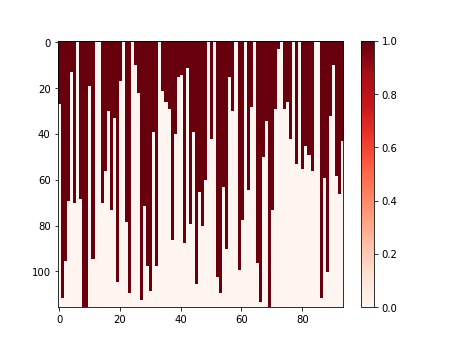
\includegraphics[width=\columnwidth]{figures/5vs7_diagonal_04_training}
                  \caption{RFNU}
                  \label{fig:Diagonal-Sample-Training-set}
        \end{subfigure}
        \begin{subfigure}[b]{0.4\linewidth}
                  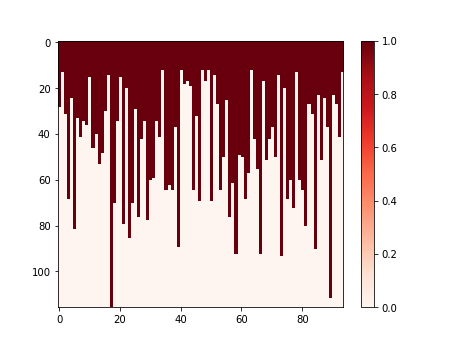
\includegraphics[width=\columnwidth]{figures/5vs7_random-triangular-largest_04_training}
                  \caption{RFNT-L}
                  \label{fig:triangular-L-Sample-Training-set}
        \end{subfigure}
        \begin{subfigure}[b]{0.4\linewidth}
                  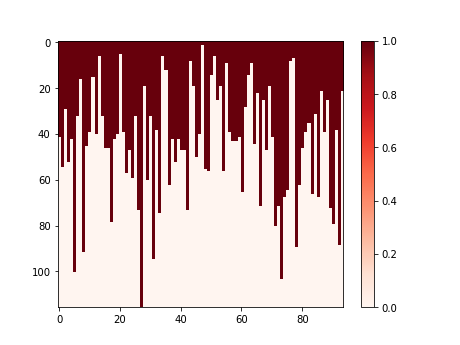
\includegraphics[width=\columnwidth]{figures/5vs7_random-triangular-smallest_04_training}
                  \caption{RFNT-S}
                  \label{fig:triangular-S-Sample-Training-set}
        \end{subfigure}
        \begin{subfigure}[b]{0.4\linewidth}
        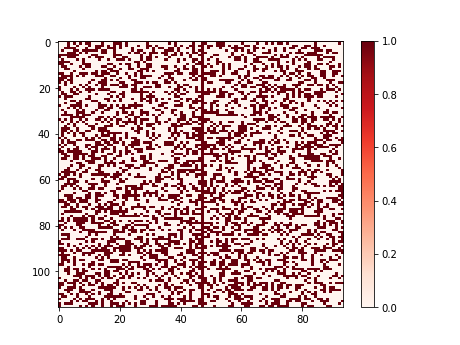
\includegraphics[width=\columnwidth]{figures/5vs7_random-unreal_04_training}
                  \caption{Random Unreal}
                  \label{fig:Random-Unreal-Sample-Training-set}
        \end{subfigure}
        \caption{Sample training set for different methods with a training ratio of 0.4.}                
\end{figure}

\paragraph{Random Subjects -- RS (Figure~\ref{fig:Uniform-S-Sample-Training-set})} This method builds the 
training set by selecting the files from random subjects 
until the training ratio is reached. The file selected in a 
subject is the file with the lowest index in this subject that has not 
been already selected in the training set. This method is realistic as 
files are sampled according to their production time-stamps. 

\paragraph{Random File Numbers (Uniform) -- RFNU (Figure~\ref{fig:Diagonal-Sample-Training-set})}
The number of files selected for every subject is randomly selected in
a uniform distribution $U(\textit{a},\textit{b})$, where \textit{b} is set to the total
number of files $N_{f}$ and \textit{a} is set according to training ratio $\alpha$ as follows:
\[
  \begin{cases}
          \textit{a} = 0      & \text{if $\alpha \leq 0.5$ }\\
          
          \textit{a} = (2\alpha - 1) N_{f} & \text{if $\alpha > 0.5$}
  \end{cases}
\]
This method is realistic as files are sampled according to their production time-stamps.
Due to sampling issues, it is possible that the actual training ratio obtained with this method
does not match the target one. We check that the difference between the target and real training ratios
was lower than 0.01.\\ 

\paragraph{Random File Numbers (Triangular) -- RFNT}
The number of files selected for every subject is randomly selected in
a triangular distribution with parameters \textit{a}, \textit{b} and 
\textit{c} as in Figure~\ref{fig:triangular}. The mean of the distribution is 
$\frac{a+b+c}{3}$. We set \textit{c} to $N_{f}$ and we set 
\textit{a} and \textit{b} with two approaches that ensure that the 
average of the distribution is $\alpha N_{f}$ ($\alpha$ is the training 
ratio):
\begin{enumerate}
        \item Largest a (RFNT-L, Figure~\ref{fig:triangular-L-Sample-Training-set}): a is set to the 
        largest possible value, i.e., b. The average of the 
        distribution is $\frac{2a+N_{f}}{3}$, therefore 
        $a=\frac{3\alpha-1}{2}N_{f}$.
                \item Smallest a (RFNT-S, Figure~\ref{fig:triangular-S-Sample-Training-set}): a is 
        set to the smallest possible value, i.e., 0. The average of the 
        distribution is $\frac{b+N_{f}}{3}$, therefore 
        $b=N_{f}(3\alpha-1)$. To ensure that $b<N_{f}$, we actually set 
        $b$ to $\min(N_{f}, N_{f}(3\alpha-1))$. 
\end{enumerate}
It should be noted that $\alpha$ must be larger than $\frac{1}{3}$ for 
a and b to remain positive. For training ratios lower than $\frac{1}{3}$, we 
define RFNT methods as the RFNU one presented previously.
As illustrated in Figures~\ref{fig:triangular-L-Sample-Training-set} 
and~\ref{fig:triangular-S-Sample-Training-set}, the motivation for the 
RFNT-L method is to guarantee that, for large enough values of 
$\alpha$, all subjects will have at least a few files in the training 
set, which is not the case for RFNU.
\begin{figure}
\centering
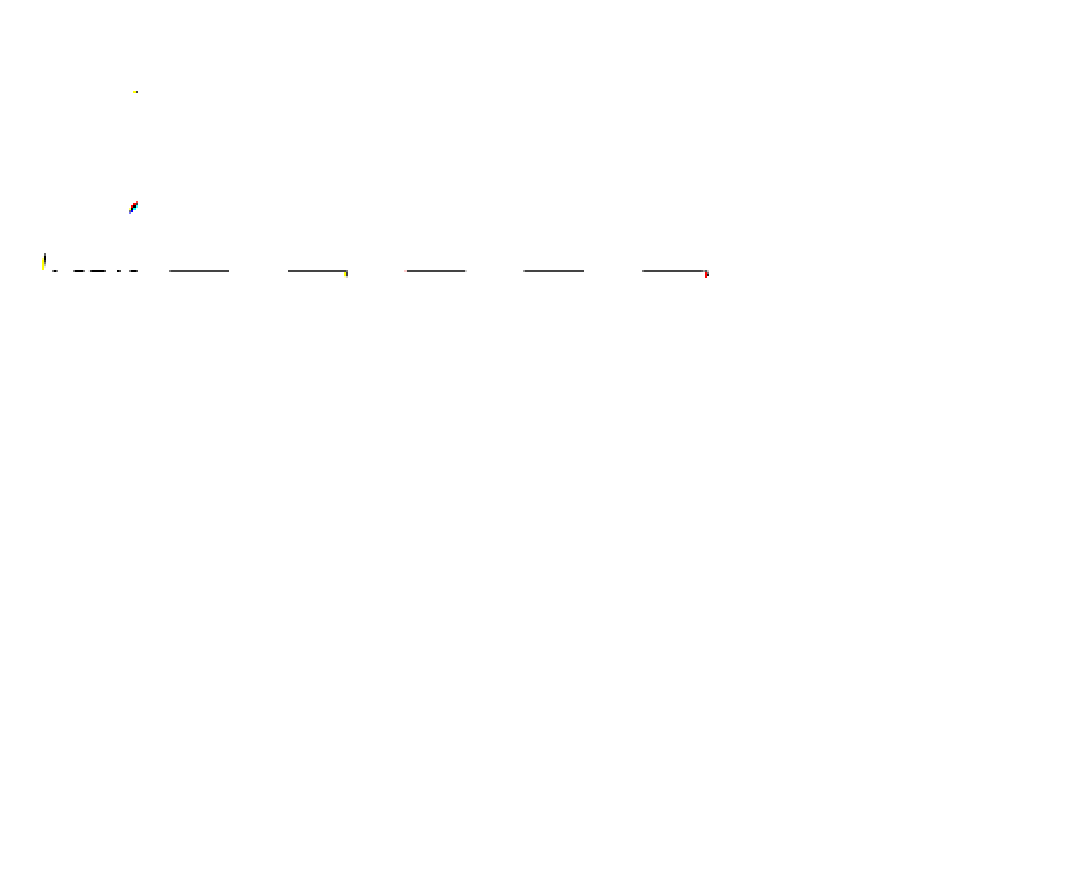
\includegraphics[width=0.5\columnwidth]{figures/triangular.pdf}
\caption{Triangular distribution}
\label{fig:triangular}
\end{figure}

% 0. random unreal (baseline)
\paragraph{Random Unreal (Figure ~\ref{fig:Random-Unreal-Sample-Training-set})}
The training set is sampled in a random uniform way, 
regardless of the file generation times. This method will be used as a
baseline for comparison with other methods, although it is not
realistic.

In each method, we also included the first row of the matrix (first 
generated file of each subject) and a random column (all files of a 
random subject) to avoid cold start issues. 


\section{Dataset}

\todo{Soudabeh, can you remove the caption on all matrices?}

\subsection{Synthetic Data}

We generated synthetic matrices as shown in 
Figure~\ref{fig:synthetic-data}. Each matrix has 100 files and 100 
subjects of different \emph{types}. Subjects of the same type behave 
identically and all types contain the same number of subjects $\pm$ 1 
\todo{Soudabeh: check that}. Such a decomposition by subject type 
correspond to the case where different subjects may have data of 
different nature, as it is for instance the case in the neuroimaging 
dataset of the Human Connectome Project~\cite{van2013wu} where not all the 
subjects have the same amount of images.

For subjects of a given type, matrix elements vary in $log(n)$  blocks,         
where $n$ is the number of types, with all the possible variation 
patterns: some types do not vary at all, while other ones vary in every 
block. Such variation patterns are meant to mimic the logic of data 
processing pipelines: each block of files represents the files produced 
at a given stage of the pipeline, which may or may not contain 
reproducibility errors depending on the subject type.

\begin{figure}
\centering
        %\begin{subfigure}[b]{0.4\linewidth}
                  %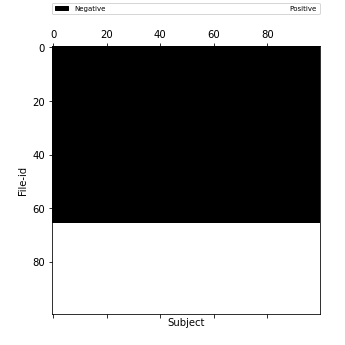
\includegraphics[width=\columnwidth]{data/Utility_Matrix/Synthetic/synthetic_subject_types/1_SubjectType_utility_matrix.png}
                  %\caption{1 type}
        %\end{subfigure}
        \begin{subfigure}[b]{0.4\linewidth}
                  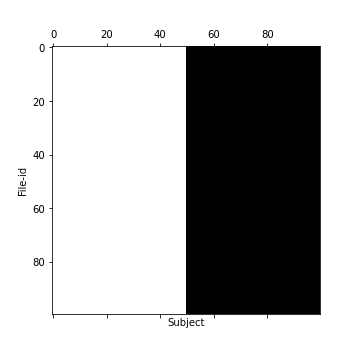
\includegraphics[width=\columnwidth]{data/Utility_Matrix/Synthetic/synthetic_subject_types/2_SubjectType_utility_matrix.png}
                  \caption{2 types}
        \end{subfigure}
        \begin{subfigure}[b]{0.4\linewidth}
                  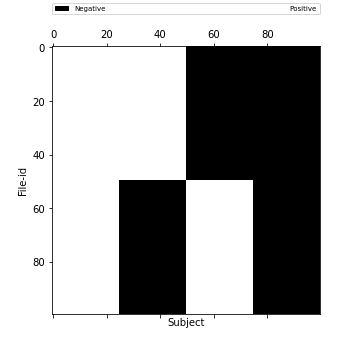
\includegraphics[width=\columnwidth]{data/Utility_Matrix/Synthetic/synthetic_subject_types/4_SubjectType_utility_matrix.png}
                  \caption{4 types}
        \end{subfigure}
                \begin{subfigure}[b]{0.4\linewidth}
                  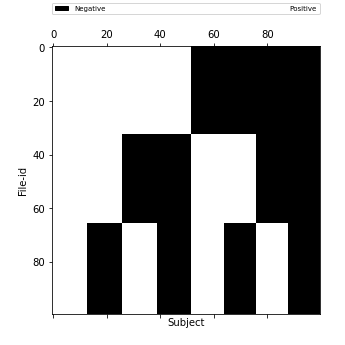
\includegraphics[width=\columnwidth]{data/Utility_Matrix/Synthetic/synthetic_subject_types/8_SubjectType_utility_matrix.png}
                  \caption{8 types}
        \end{subfigure}
                \begin{subfigure}[b]{0.4\linewidth}
                  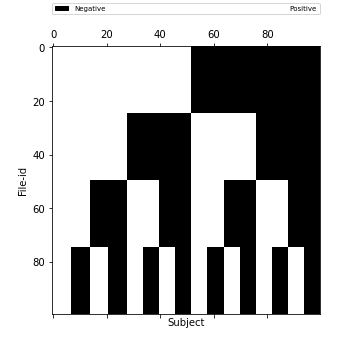
\includegraphics[width=\columnwidth]{data/Utility_Matrix/Synthetic/synthetic_subject_types/16_SubjectType_utility_matrix.png}
                  \caption{16 types}
        \end{subfigure}
                \begin{subfigure}[b]{0.4\linewidth}
                  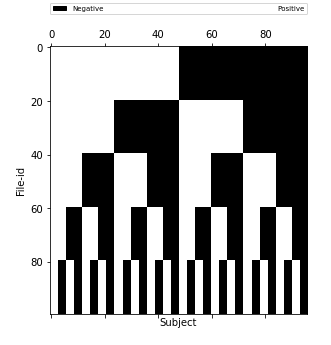
\includegraphics[width=\columnwidth]{data/Utility_Matrix/Synthetic/synthetic_subject_types/32_SubjectType_utility_matrix.png}
                  \caption{32 types}
        \end{subfigure}
                \begin{subfigure}[b]{0.4\linewidth}
                  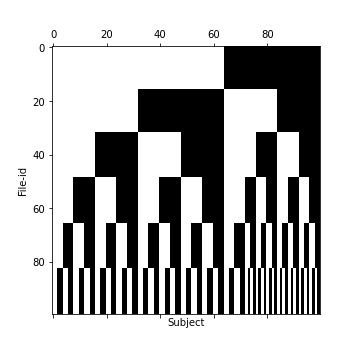
\includegraphics[width=\columnwidth]{data/Utility_Matrix/Synthetic/synthetic_subject_types/64_SubjectType_utility_matrix.png}
                  \caption{64 types}
        \end{subfigure}
\caption{Synthetic Data}
\label{fig:synthetic-data}
\end{figure}

\subsection{Real Data}

We collected data to evaluate the computational reproducibility of analysis
pipelines of the Human Connectome Project~\cite{glasser2013minimal}. We
processed a set S of 94 subjects randomly selected in the S500 HCP
release~\todo{URL} in three execution conditions with different
versions of the CentOS operating system (5.?, 6.? and 7.?), using the
PreFreesurfer and Freesurfer pipelines
described in~\cite{glasser2013minimal} and available at \todo{URL}. For
each pipeline, we identified the set F of files produced for all
subjects in all conditions. For each condition pair and each pipeline,
we computed a binary difference matrix D of size $|F|\times|S|$, where $D_{i,j}$ is true
if file $i$ of subject $j$ was different in each condition. Rows of
$M$ are ordered by ascending file modification time in the pipeline.

Figure~\ref{fig:utility-matrices} shows the utility matrices
obtained for the PreFreesurfer and Freesufer pipeline. The computational
reproducibility of these pipelines varies across subjects,
but some files behave
consistently across all subjects, leading to complete black or white
lines.
%The ratio of positive elements in utility matrix of CentOS5 vs CentOS6(C5C6),  CentOS5 vs CentOS7(C5C7) and  CentOS6 vs CentOS7(C6C7) are
%$0.34$, $0.79$ and $0.79$ respectively.

\begin{figure}[h!]
  \centering
  \begin{subfigure}[b]{0.45\linewidth}
        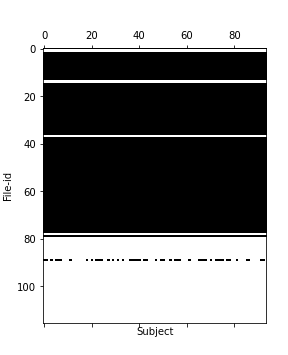
\includegraphics[width=\columnwidth]{data/Utility_Matrix/PreFreeSurfer/PFS_5v6_utility_matrix.png}
  \caption{PFS, C5 vs C6}
  \end{subfigure}
  \begin{subfigure}[b]{0.45\linewidth}
         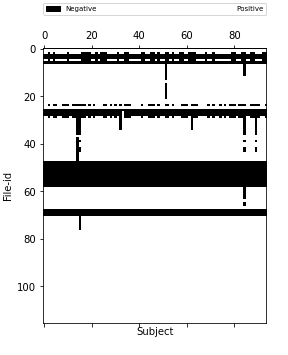
\includegraphics[width=\columnwidth]{data/Utility_Matrix/PreFreeSurfer/PFS_5v7_utility_matrix.png}
  \caption{PFS, C5 vs C7}
  \end{subfigure}
  \begin{subfigure}[b]{0.45\linewidth}
        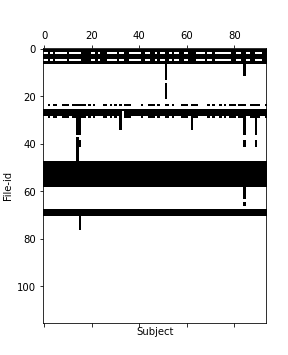
\includegraphics[width=\columnwidth]{data/Utility_Matrix/PreFreeSurfer/PFS_6v7_utility_matrix.png}
  \caption{PFS, C6 vs C7}
  \end{subfigure}
  \begin{subfigure}[b]{0.45\linewidth}
        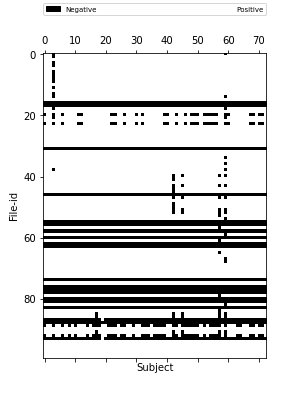
\includegraphics[width=\columnwidth]{data/Utility_Matrix/FS-100files/FS-First-bound-100files.png}
  \caption{FS (first 100 files), C6 vs C7}
  \end{subfigure}
  \caption{Utility matrices, PreFreesurfer (PFS) and Freesurfer (FS) pipelines}
    \label{fig:utility-matrices}
\end{figure}


\section{Results}


Three experiments have been conducted for each dataset to evaluate the performance of our 
predictions using (1) ALS without biases, (2) ALS with biases, (3) Biases only. 
Results will be evaluated using accuracy, sensitivity and specificity defined as follows:
\[
        Accuracy = \frac{TP+TN}{TP+TN+FP+FN}
\]
\[
        Sensitivity = \frac{TP}{TP+FN}
\]
\[
        Specificity = \frac{TN}{TN+FP}
\]
Where TP is the number of True Positives (correctly predicted reproducibility errors), 
FP is the number of False Positives, TN is the number of true negatives 
and FN is the number of false negatives. \todo{Check if we want to report sensitivity and specificity, otherwise remove.}

We compare our sampling methods to (1) a dummy classifier that always predicts the value in the majority class
 and (2) the Random Unreal method, used as the baseline sampling technique.

\subsection{Synthetic Data}

\subsubsection{ALS without Bias}

Accuracy results for the different numbers of subject types are 
reported in Figure~\ref{fig:results-synthetic}. By construction, the 
accuracy of the dummy classifier is 0.5 for all subject types. Random 
Unreal performs very well for all subject types, which confirms that 
ALS is working correctly. Unsurprisingly, all the other methods perform 
better than the dummy classifier, and their accuracy decreases as the 
number of subject types increases.

However, only 3 methods are able to provide accuracy values above 0.85 
for all subject types: Random Subjects (RS), RFNU and RFNTL. This is 
due to the fact that these methods are the only ones that can sample 
files produced toward the end of the execution while maintaining a 
reduced number of empty columns. Surprisingly, RFNTS does not perform 
well for more than 2 subject types \todo{Check that.}.

RS, RFNU and RFNTL achieve a 90\% accuracy for a training ratio of 
about 0.85. Therefore, 15\% of the computations could potentially be 
saved in such reproducibility studies.

\begin{figure*}
\begin{subfigure}[b]{0.4\linewidth}
        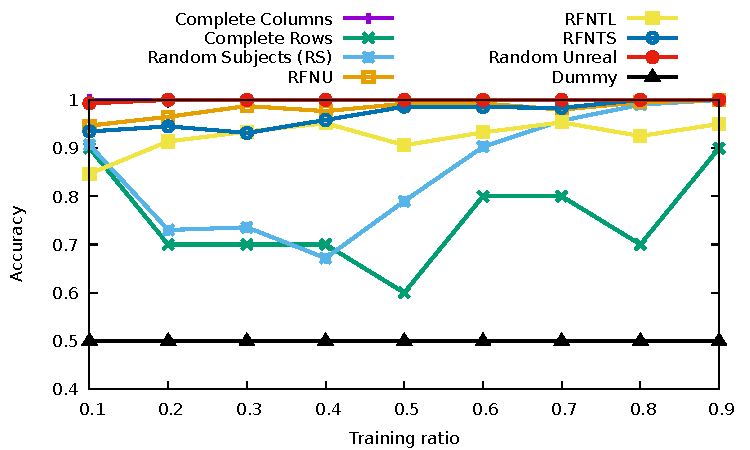
\includegraphics[width=0.8\columnwidth, angle=-90]{data/results/means_of_results/ALS/Synthetic/synthetic_subject_types/ALS-2-types.pdf}
        \caption{2 subject types}
\end{subfigure}
\begin{subfigure}[b]{0.4\linewidth}
        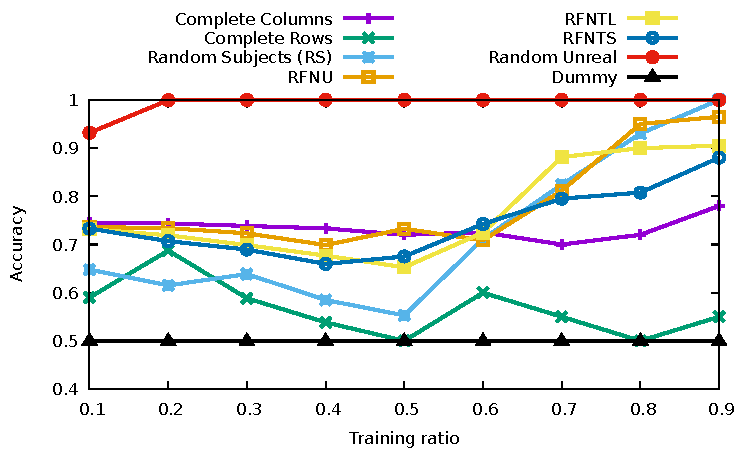
\includegraphics[width=0.8\columnwidth, angle=-90]{data/results/means_of_results/ALS/Synthetic/synthetic_subject_types/ALS-4-types.pdf}
        \caption{4 subject types}
\end{subfigure}
\begin{subfigure}[b]{0.4\linewidth}
        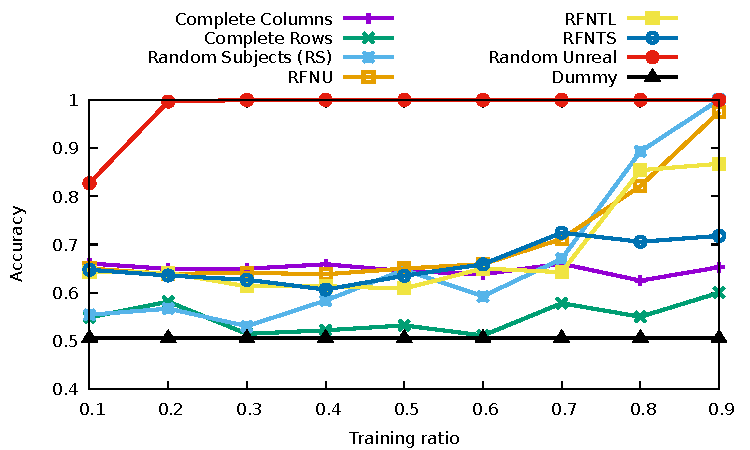
\includegraphics[width=0.8\columnwidth, angle=-90]{data/results/means_of_results/ALS/Synthetic/synthetic_subject_types/ALS-8-types.pdf}
        \caption{8 subject types}
\end{subfigure}
\begin{subfigure}[b]{0.4\linewidth}
        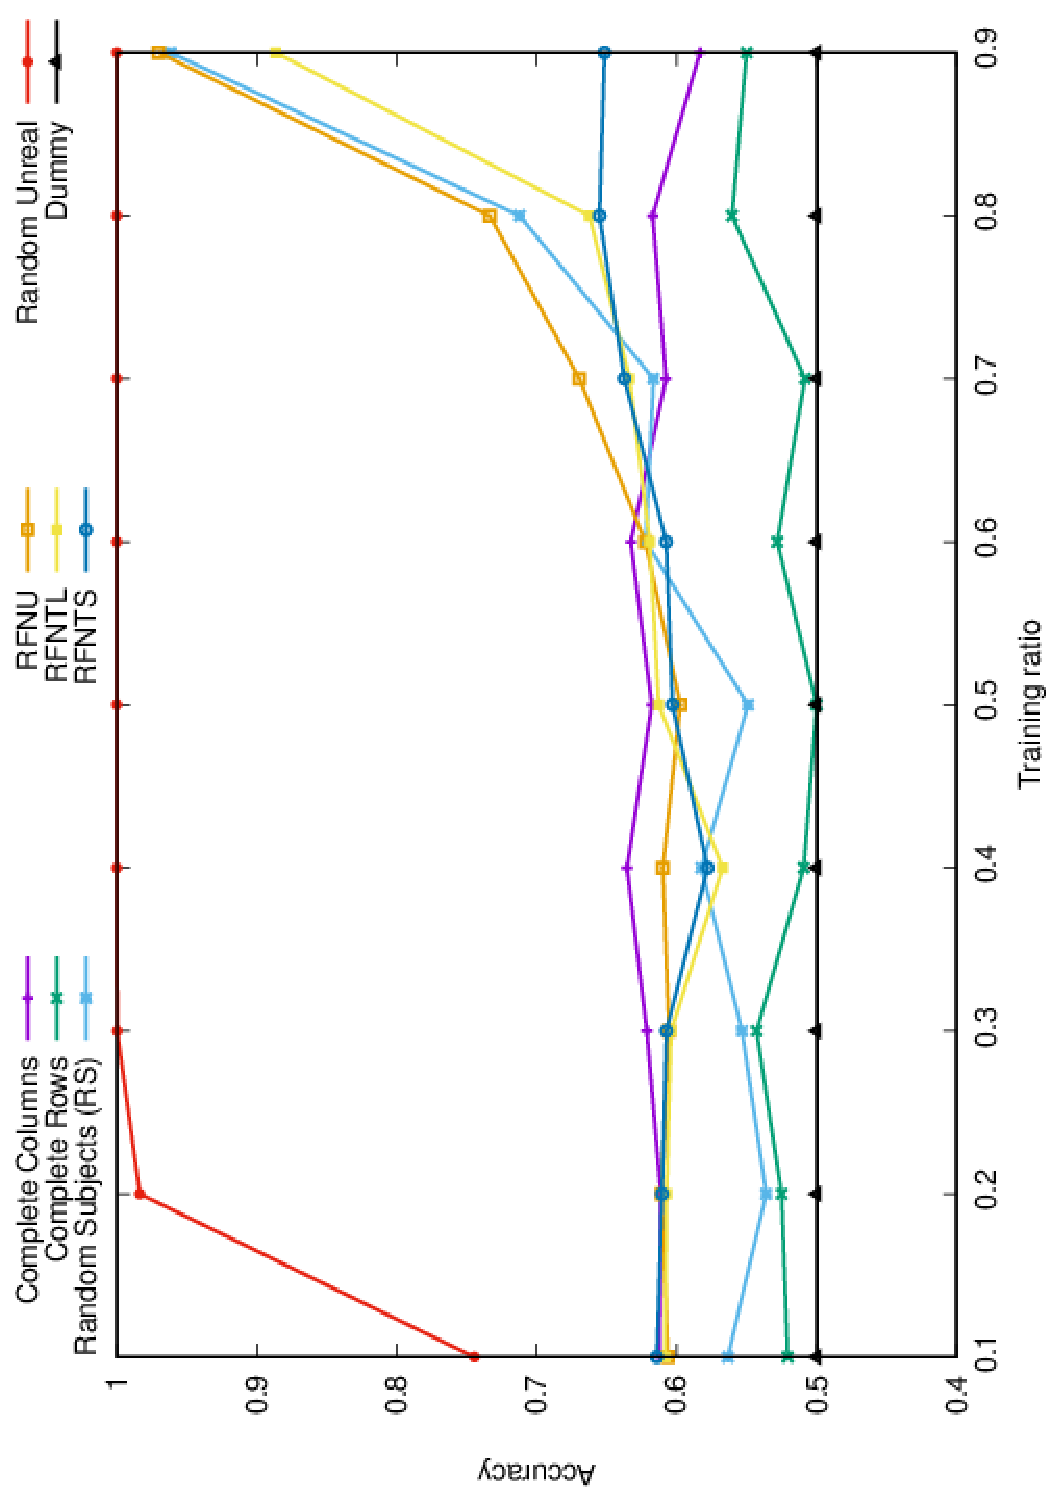
\includegraphics[width=0.8\columnwidth, angle=-90]{data/results/means_of_results/ALS/Synthetic/synthetic_subject_types/ALS-16-types.pdf}
        \caption{16 subject types}
\end{subfigure}
\begin{subfigure}[b]{0.4\linewidth}
        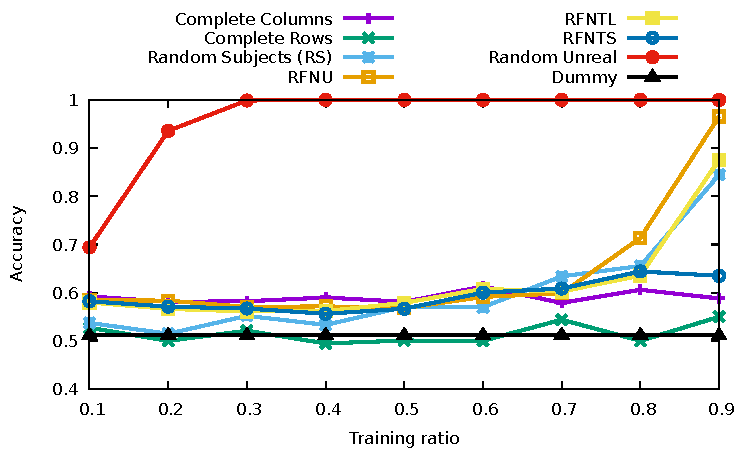
\includegraphics[width=0.8\columnwidth, angle=-90]{data/results/means_of_results/ALS/Synthetic/synthetic_subject_types/ALS-32-types.pdf}
        \caption{32 subject types}
\end{subfigure}
\hfill
\begin{subfigure}[b]{0.4\linewidth}
        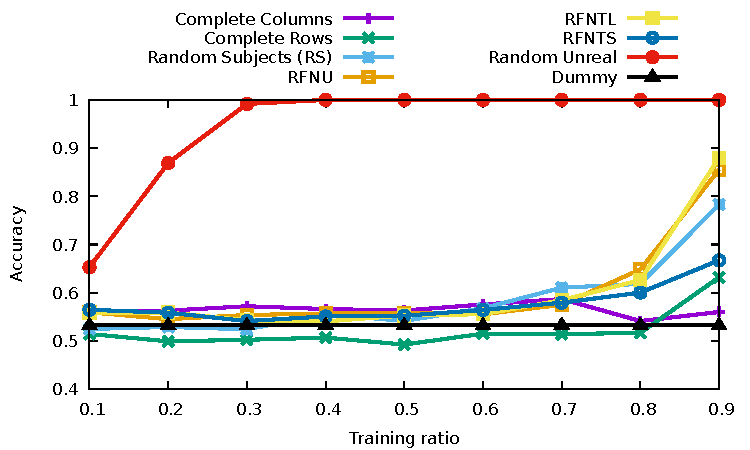
\includegraphics[width=0.8\columnwidth, angle=-90]{data/results/means_of_results/ALS/Synthetic/synthetic_subject_types/ALS-64-types.pdf}
        \caption{64 subject types}
\end{subfigure}
\caption{Accuracy results on synthetic data, ALS \emph{without} bias.}
\label{fig:results-synthetic}
\end{figure*}

\subsubsection{ALS with Bias}

Results of ALS with Bias are reported in Figure~\ref{fig:results-synthetic-als-bias}.
RS, RFNU and RFNTL remain the methods that best compare to Random Unreal, but the achieved
accuracy is much lower than without Biases. This is due to the fact that biases \ldots \todo{finish that.}

\begin{figure*}
\begin{subfigure}[b]{0.4\linewidth}
        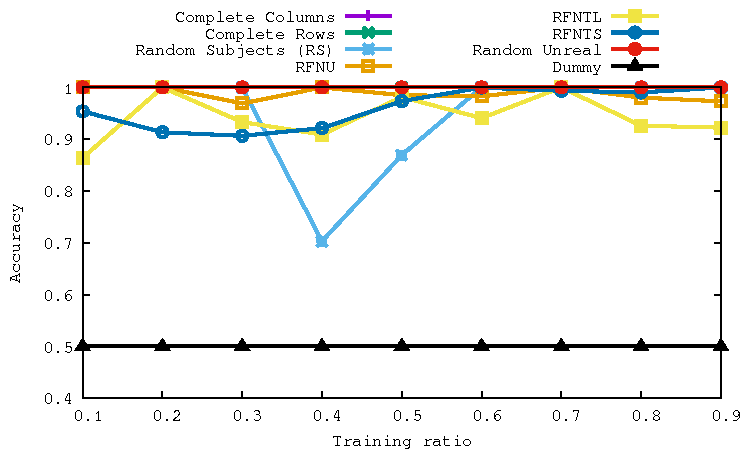
\includegraphics[width=0.8\columnwidth, angle=-90]{data/results/means_of_results/ALS-Bias/Synthetic/synthetic_subject_types/ALS-Bias-2-types.pdf}
        \caption{2 subject types}
\end{subfigure}
\begin{subfigure}[b]{0.4\linewidth}
        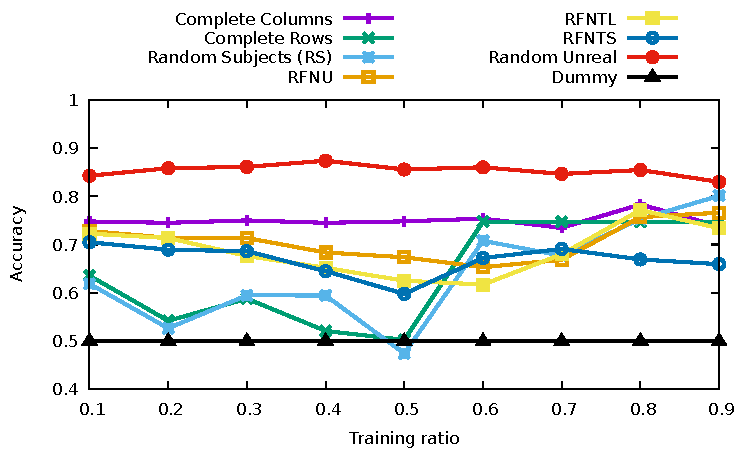
\includegraphics[width=0.8\columnwidth, angle=-90]{data/results/means_of_results/ALS-Bias/Synthetic/synthetic_subject_types/ALS-Bias-4-types.pdf}
        \caption{4 subject types}
\end{subfigure}
\begin{subfigure}[b]{0.4\linewidth}
        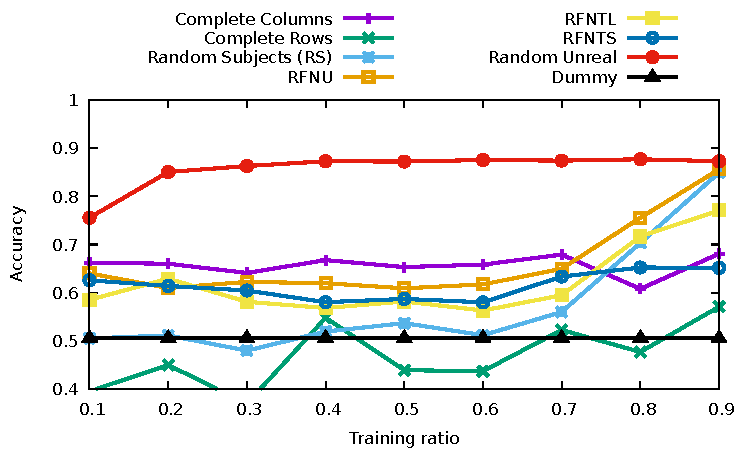
\includegraphics[width=0.8\columnwidth, angle=-90]{data/results/means_of_results/ALS-Bias/Synthetic/synthetic_subject_types/ALS-Bias-8-types.pdf}
        \caption{8 subject types}
\end{subfigure}
\begin{subfigure}[b]{0.4\linewidth}
        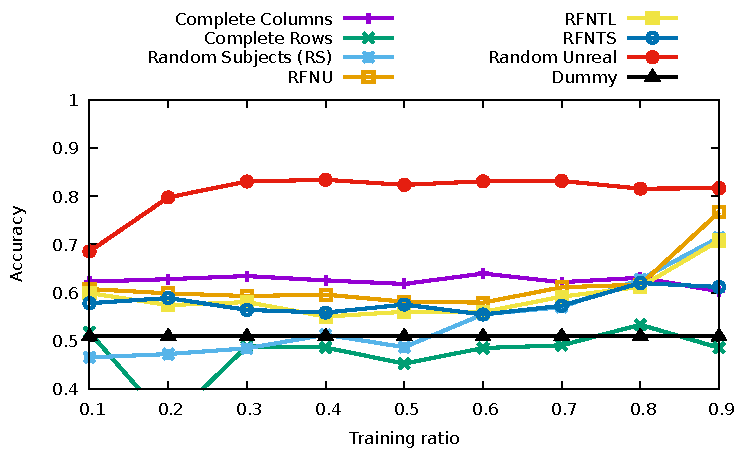
\includegraphics[width=0.8\columnwidth, angle=-90]{data/results/means_of_results/ALS-Bias/Synthetic/synthetic_subject_types/ALS-Bias-16-types.pdf}
        \caption{16 subject types}
\end{subfigure}
\begin{subfigure}[b]{0.4\linewidth}
        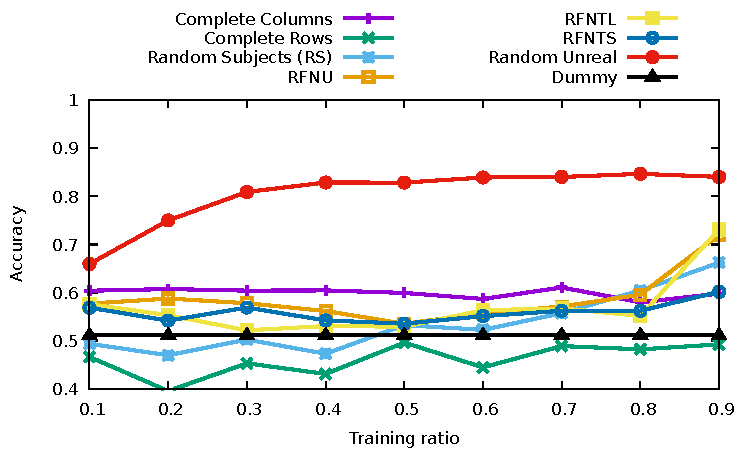
\includegraphics[width=0.8\columnwidth, angle=-90]{data/results/means_of_results/ALS-Bias/Synthetic/synthetic_subject_types/ALS-Bias-32-types.pdf}
        \caption{32 subject types}
\end{subfigure}
\hfill
\begin{subfigure}[b]{0.4\linewidth}
        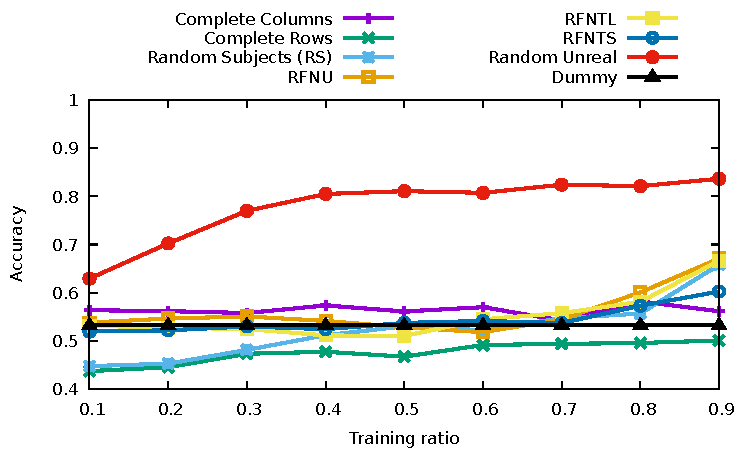
\includegraphics[width=0.8\columnwidth, angle=-90]{data/results/means_of_results/ALS-Bias/Synthetic/synthetic_subject_types/ALS-Bias-64-types.pdf}
        \caption{64 subject types}
\end{subfigure}
\caption{Accuracy results on synthetic data, ALS \emph{with} bias.}
\label{fig:results-synthetic-als-bias}
\end{figure*}

\subsection{Real Data}

\subsubsection{ALS without bias}

\begin{figure*}
\begin{subfigure}[b]{0.4\linewidth}
        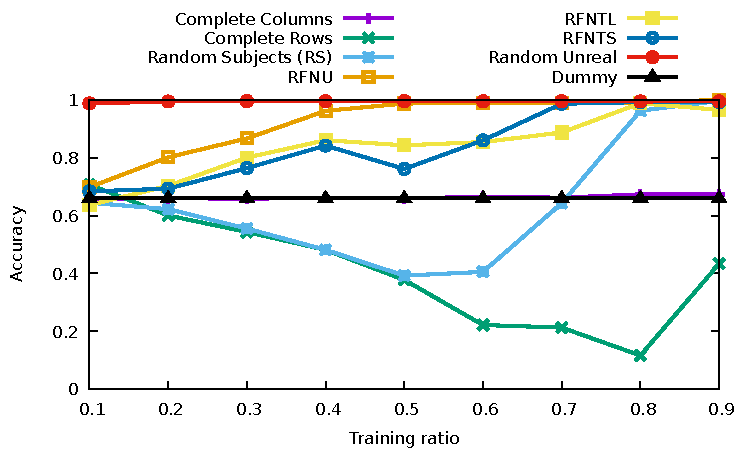
\includegraphics[width=0.8\columnwidth, angle=-90]{data/results/means_of_results/ALS/PreFreeSurfer/ALS-PFS-5v6.pdf}
        \caption{PFS, CentOS5 vs CentOS6}
\end{subfigure}
\begin{subfigure}[b]{0.4\linewidth}
        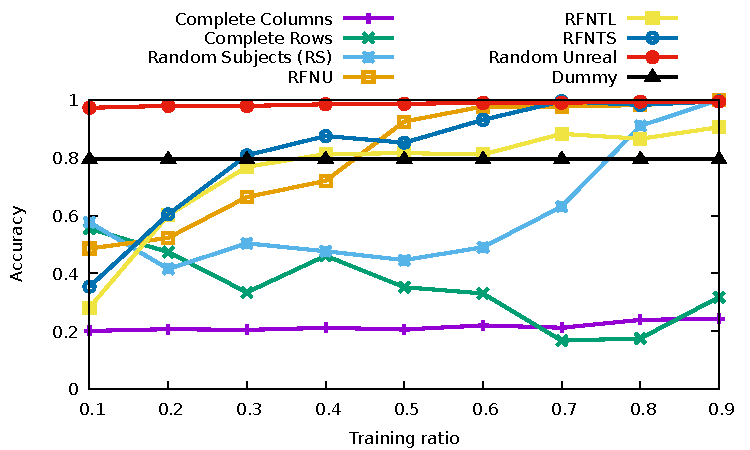
\includegraphics[width=0.8\columnwidth, angle=-90]{data/results/means_of_results/ALS/PreFreeSurfer/ALS-PFS-5v7.pdf}
        \caption{PFS, CentOS5 vs CentOS7}
\end{subfigure}
\begin{subfigure}[b]{0.4\linewidth}
        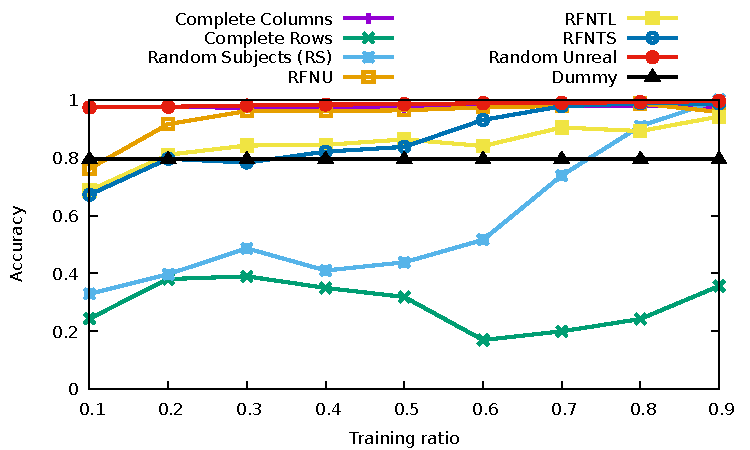
\includegraphics[width=0.8\columnwidth, angle=-90]{data/results/means_of_results/ALS/PreFreeSurfer/ALS-PFS-6v7.pdf}
        \caption{PFS, CentOS6 vs CentOS7}
\end{subfigure}\hfill
\begin{subfigure}[b]{0.4\linewidth}
        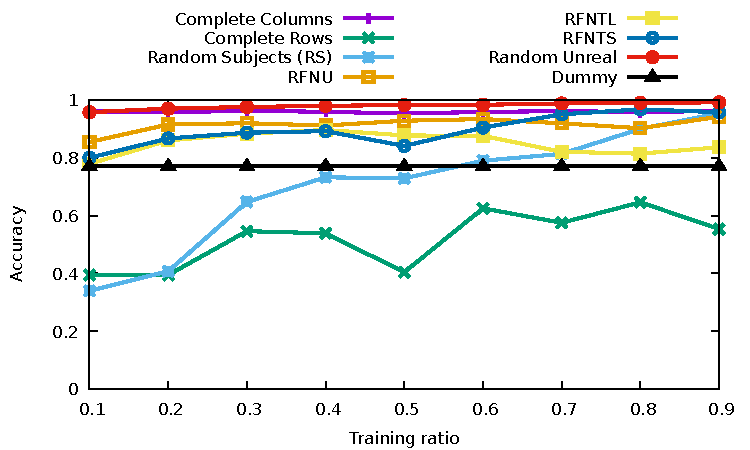
\includegraphics[width=0.8\columnwidth, angle=-90]{data/results/means_of_results/ALS/FS-100files/ALS-FS100files.pdf}
        \caption{FS, CentOS6 vs CentOS7}
\end{subfigure}
\caption{Accuracy results on PreFresurfer (PFS) and Freesurfer (FS) data, ALS \emph{without} bias.}
\label{fig:results-real-als}
\end{figure*}

\subsubsection{ALS with bias}

\begin{figure*}
\begin{subfigure}[b]{0.4\linewidth}
        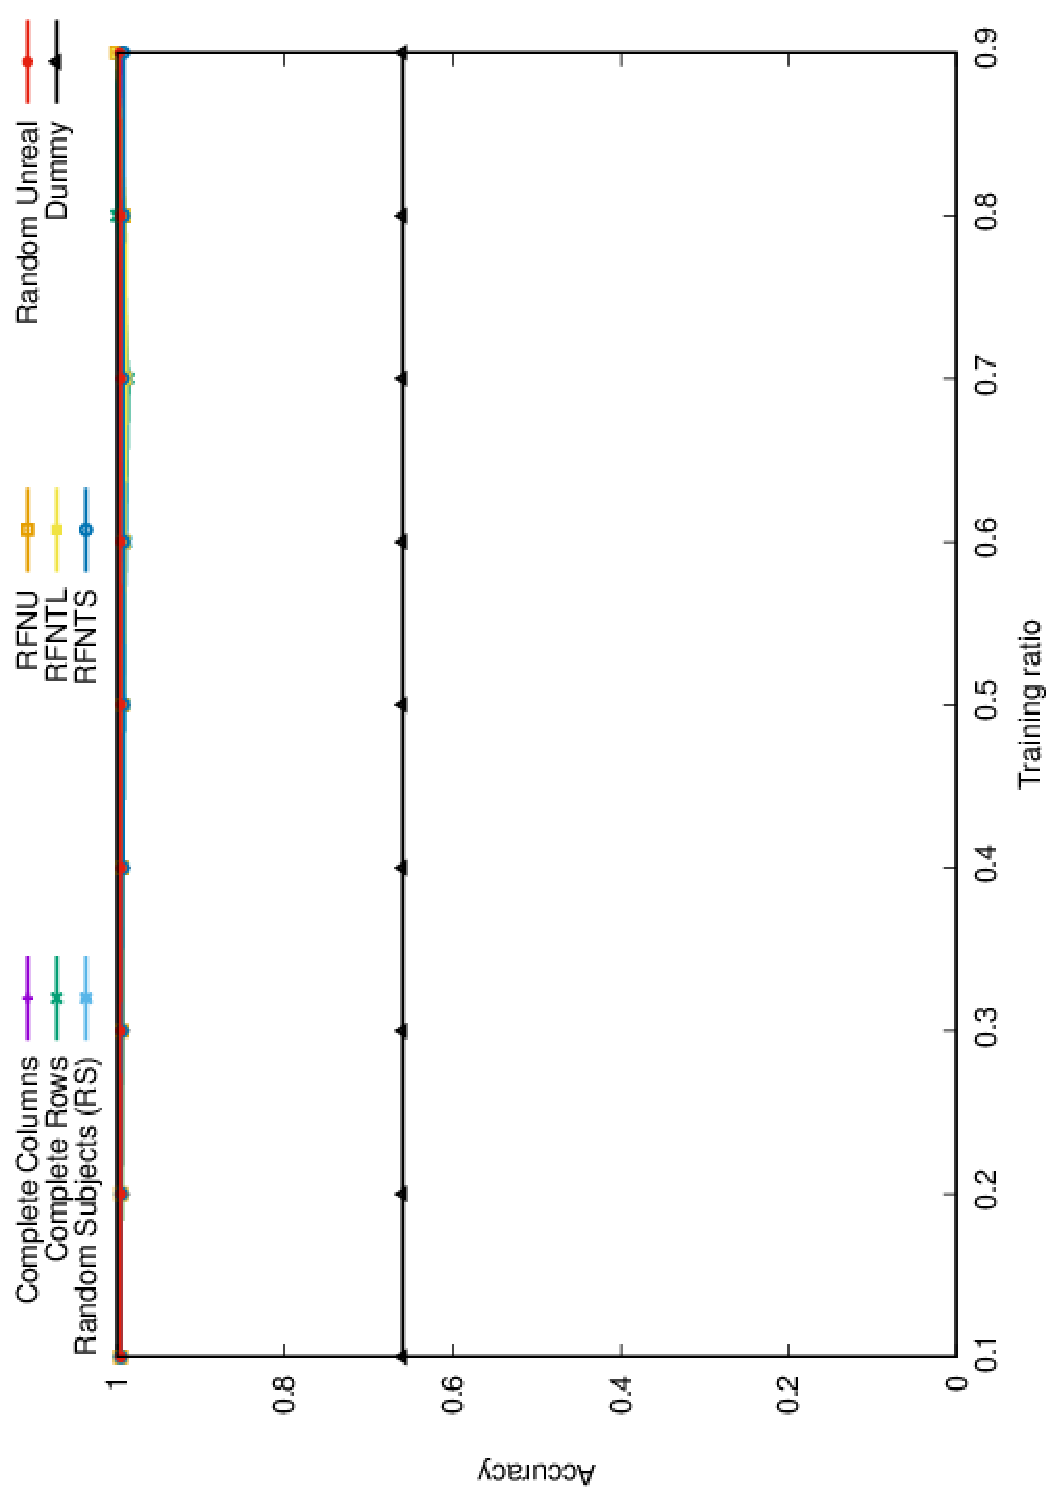
\includegraphics[width=0.8\columnwidth, angle=-90]{data/results/means_of_results/ALS-Bias/PreFreeSurfer/ALS-Bias-PFS-5v6.pdf}
        \caption{PFS, CentOS5 vs CentOS6}
\end{subfigure}
\begin{subfigure}[b]{0.4\linewidth}
        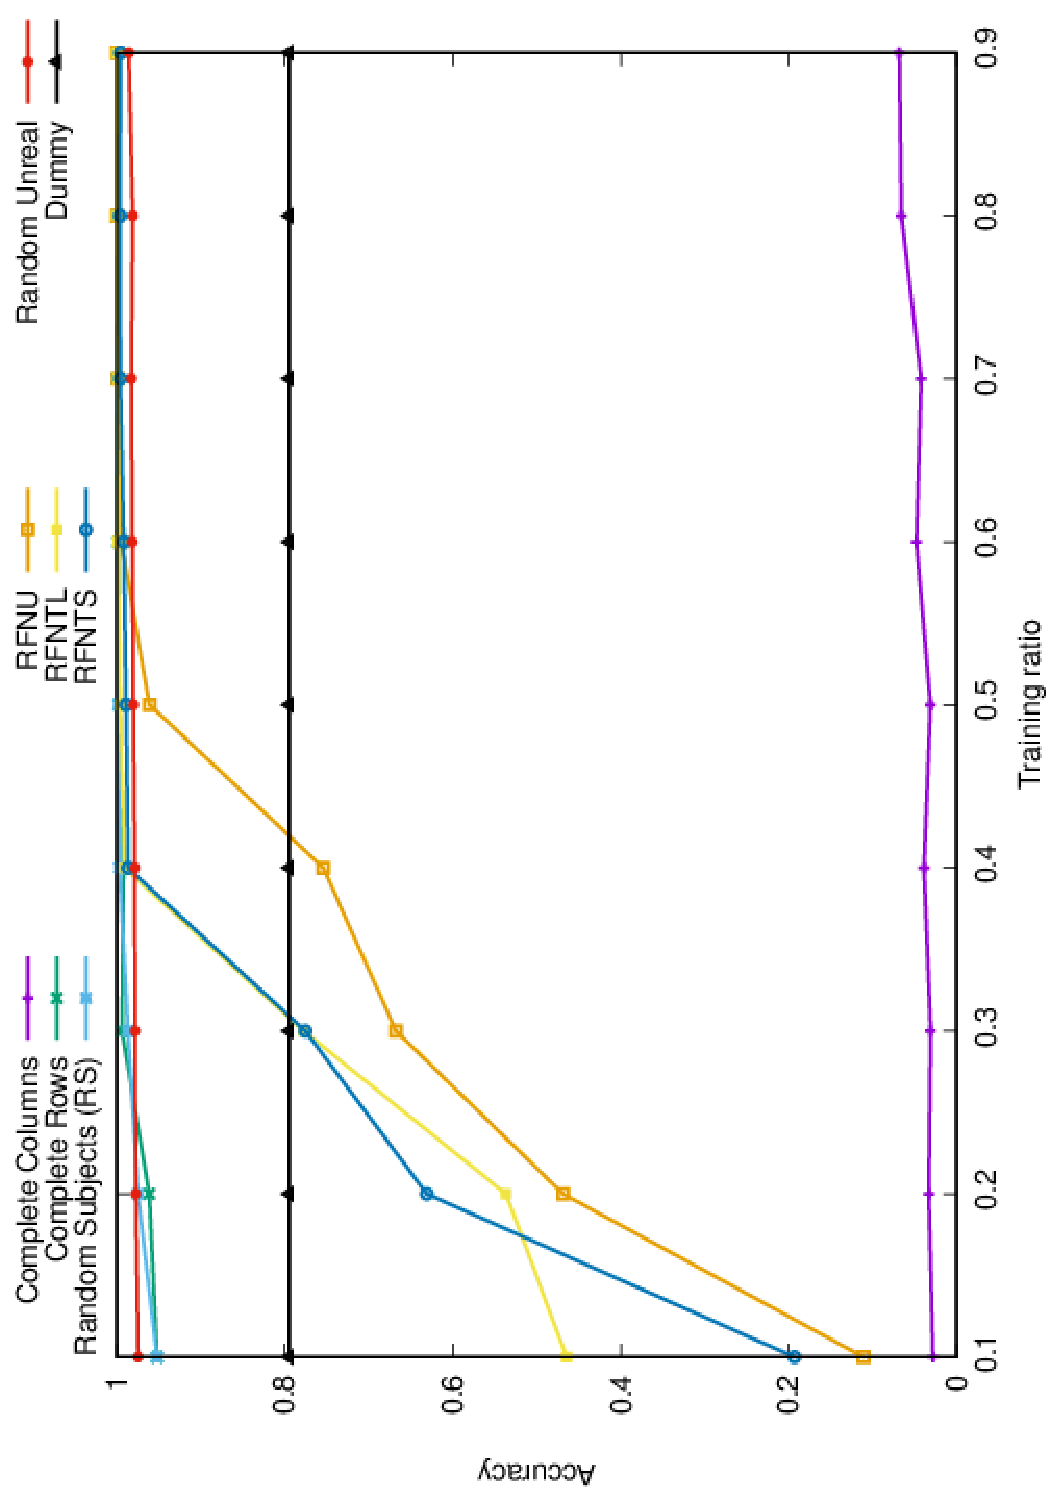
\includegraphics[width=0.8\columnwidth, angle=-90]{data/results/means_of_results/ALS-Bias/PreFreeSurfer/ALS-Bias-PFS-5v7.pdf}
        \caption{PFS, CentOS5 vs CentOS7}
\end{subfigure}
\begin{subfigure}[b]{0.4\linewidth}
        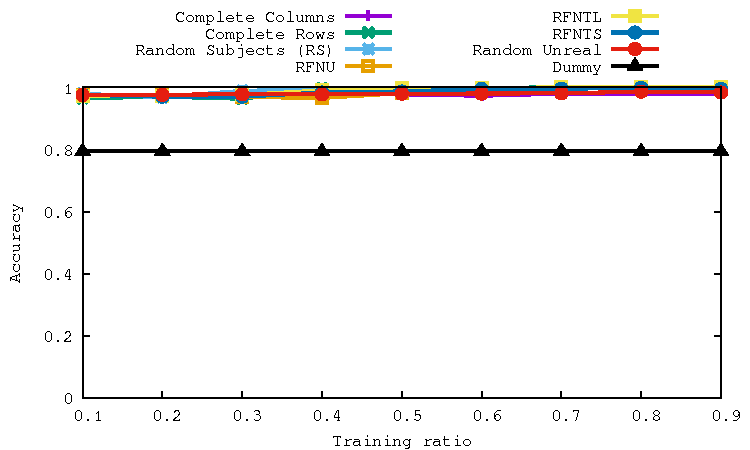
\includegraphics[width=0.8\columnwidth, angle=-90]{data/results/means_of_results/ALS-Bias/PreFreeSurfer/ALS-Bias-PFS-6v7.pdf}
        \caption{PFS, CentOS6 vs CentOS7}
\end{subfigure}\hfill
\begin{subfigure}[b]{0.4\linewidth}
        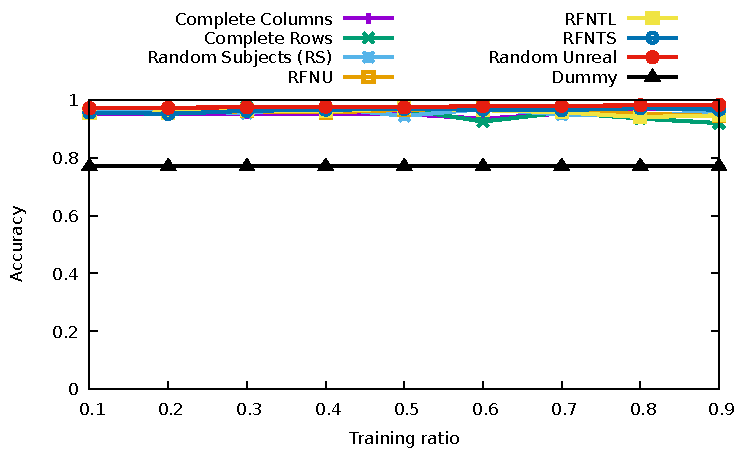
\includegraphics[width=0.8\columnwidth, angle=-90]{data/results/means_of_results/ALS-Bias/FS-100files/ALS-Bias-FS100files.pdf}
        \caption{FS, CentOS6 vs CentOS7}
\end{subfigure}
\caption{Accuracy results on PreFresurfer (PFS) and Freesurfer (FS) data, ALS \emph{with} bias.}
\label{fig:results-real-als-bias}
\end{figure*}

 
%%%%%%%%%%%%%%%%%%%%%%%%%%%%%%%%%%%%%%%%%%%%%%%%%%%
% General conclution on results of ALS without Bias 
%~ In general the accuracy pattern of the two Complete Rows and 
%~ RS methods show similar decline and grow behaviour over the 
%~ training ratio axis however it can be subject to considerable 
%~ fluctuations in differentiated condition pairs. Despite of their 
%~ likely irrational behaviour, they always have better accuracy 
%~ for the training size with less than $0.3$ in comparison to other 
%~ methods. This better performance (around 75 percent)is almost three 
%~ times higher than other methods in condition pairs with more 
%~ differences but just 20 percent better when the conditions are more 
%~ similar to each other (CentOS5 vs CentOS6) with accuracy of $90\%$.
%~ Figure~\ref{fig:RS_Rows} represents
%~ the accuracy graph of these two methods with comparison to dummy
%~ classifier over the increment of the training ratio.
%~ \begin{figure}[h!]
        %~ \centering
        %~ \begin{subfigure}[b]{0.4\linewidth}
                %~ 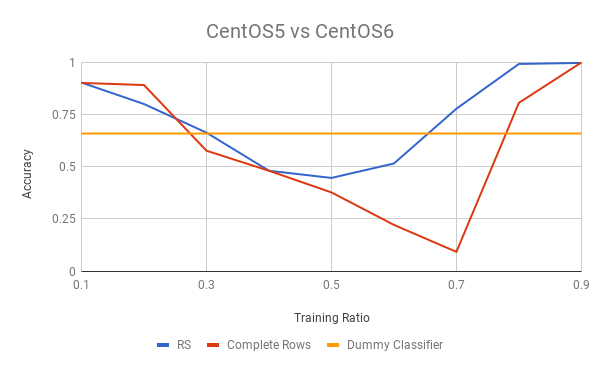
\includegraphics[width=\columnwidth]{figures/RS_Rows_5vs6}
        %~ \end{subfigure}
        %~ \begin{subfigure}[b]{0.4\linewidth}
                %~ 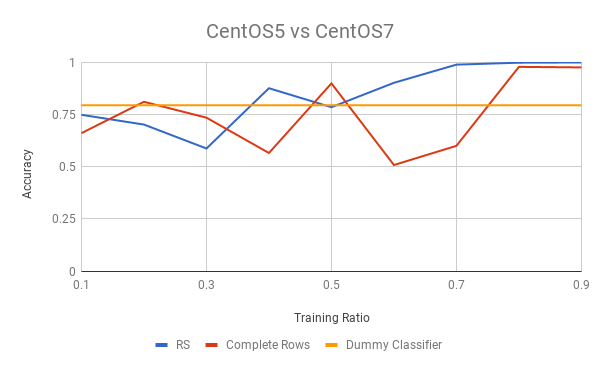
\includegraphics[width=\columnwidth]{figures/RS_Rows_5vs7}
        %~ \end{subfigure}
        %~ \begin{subfigure}[b]{0.4\linewidth}
                %~ 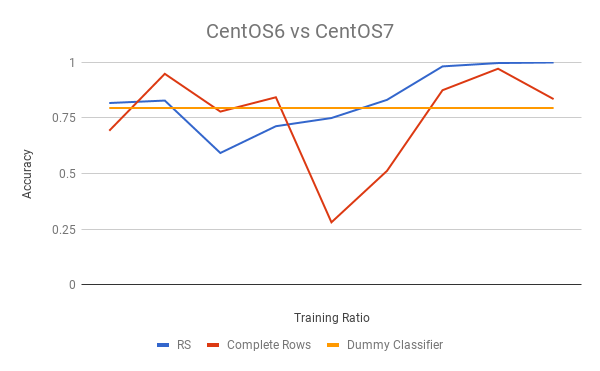
\includegraphics[width=\columnwidth]{figures/RS_Rows_6vs7}
        %~ \end{subfigure}
        %~ \caption{Average performance of RS and Complete Rows methods in three different condition pairs}
        %~ \label{fig:RS_RowS}
%~ \end{figure}

%~ All the other random methods, RS and both RFNT approaches 
%~ are performing a continues growth Figure~\ref{fig:simple-methods} represents
%~ the accuracy graph of all random methods with comparison to dummy
%~ classifier over the increment of the training ratio.. Although some considerable variation 
%~ for both triangular approaches have been observed (CentOS5 vs CentOS6) 
%~ their constant rise leads us to the next phase of experiments which was 
%~ adding up bias into the current ALS technique. 
%~ The training set suffers from lacking the files which are almost generated towards the end of pipeline.

%~ \begin{figure}[h!]
        %~ \centering
        %~ \begin{subfigure}[b]{0.4\linewidth}
                %~ 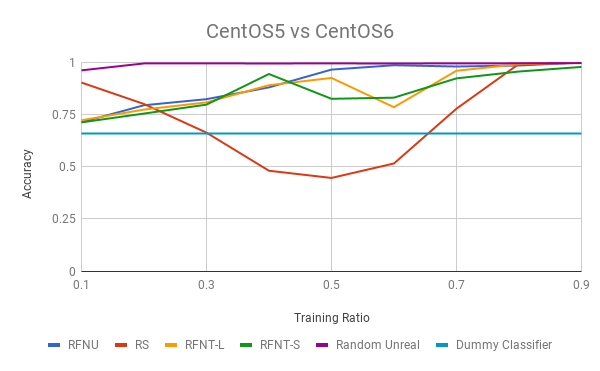
\includegraphics[width=\columnwidth]{figures/simple-methods-5vs6}
        %~ \end{subfigure}
        %~ \begin{subfigure}[b]{0.4\linewidth}
                %~ 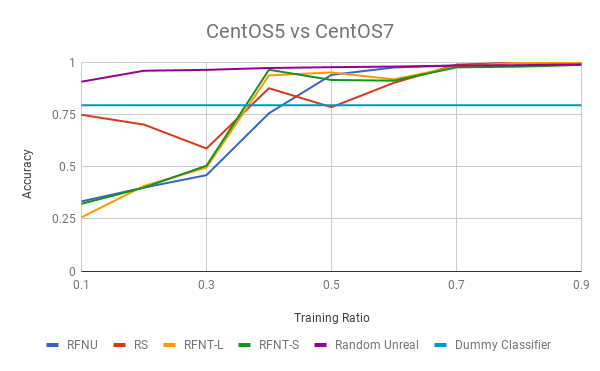
\includegraphics[width=\columnwidth]{figures/simple-methods-5vs7}
        %~ \end{subfigure}
        %~ \begin{subfigure}[b]{0.4\linewidth}
                %~ 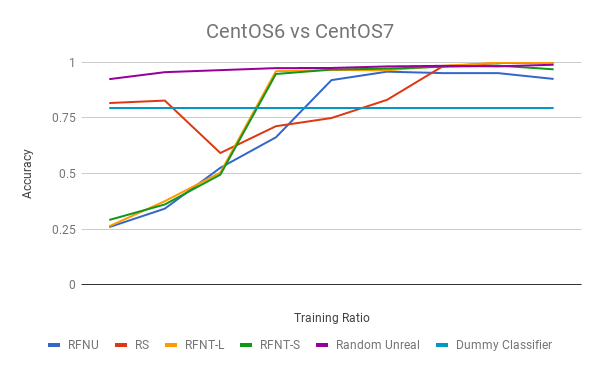
\includegraphics[width=\columnwidth]{figures/simple-methods-6vs7}
        %~ \end{subfigure}
        %~ \caption{Average performance of all methods in three different condition pairs}
        %~ \label{fig:simple-methods}
%~ \end{figure}





%-----------------------------------------------------------
% Present your results: accuracy, ROC curves, transparency matrix, factors. 

% Try with different numbers of factors. 

\section{Discussion}
this is just a test of compiling 

% Not all subjects behave the same, which motivates the Big Data approach. 

% Which sampling method is best

% Interpreting the factors? Factors reflect the pipeline definition. 

% How can this be used in practice

% What are the limitations

% Real values, we expect the best sampling method to remain the same.

\section{Conclusion}

% Summary of the results and discussion. The take-home message.
%%%%%% why there is a drop in ALS-RFNT-L with 60% ratio?  

\todo{Make sure the code is available and results are reproducible.}

\section*{Acknowledgement}

\bibliographystyle{IEEEtran}
\bibliography{IEEEabrv,biblio.bib}


\end{document}
